\documentclass[10pt]{article}
\usepackage[letterpaper,margin=0.8in]{geometry}
\usepackage[T1]{fontenc}
\usepackage{lmodern,microtype,booktabs,graphicx,tabularx,array,float,caption}
\usepackage[hidelinks]{hyperref}
\renewcommand{\arraystretch}{1.15}
\setlength{\parindent}{0pt}\setlength{\parskip}{4pt}
\begin{document}
{\Large\bfseries Claude Fable 5.1 on mcbench: run19-v2}\\[2pt]
Minecraft, pixels only. Run date 2026-10-19.

\section*{Setup}
\begin{itemize}\itemsep0pt
\item Model: \texttt{claude-fable-5-1} through \texttt{claude -p} on a Claude subscription (every reply checked to come from this model).
\item 19 tasks, one episode each (dev seed 1 of each task), charged mode: the game keeps running while Fable thinks, with its previous action still applied.
\item Fable sees one 640$\times$360 screenshot, the goal sentence, elapsed game time, its last 5 actions, and how long its last think took. Prompt \texttt{mcbench-fable-prompt v3}.
\item Each action can set a duration (up to 5 s); after it runs out the player stands still until the next action.
\item Cap of 100 Fable calls per episode (never reached). 171 calls in total for these episodes, 0 unreadable replies.
\item \texttt{collect\_wood} was left out: breaking the bottom log leaves the rest of the log pillar floating out of reach.
\end{itemize}

\section*{Summary}
Fable passed \textbf{3 of 19} tasks. With one episode per task, these numbers are a rough picture, not a precise rate.

\begin{table}[H]\centering
\begin{tabular}{lcc}\toprule
Category & Passed & Tasks \\\midrule
navigation & 0 & 3 \\
combat & 0 & 3 \\
survival & 0 & 3 \\
manipulation & 2 & 2 \\
exploration & 1 & 2 \\
planning & 0 & 4 \\
adaptation & 0 & 2 \\
\midrule
total & 3 & 19 \\\bottomrule
\end{tabular}\end{table}

\textbf{Patterns.}
\begin{itemize}\itemsep0pt
\item \textbf{Too slow for fights.} A think takes about 2.5--4 s; a zombie or skeleton deals enough damage in 3--4 thinks to kill Fable. All 6 combat and survival episodes ended in death or a lost target.
\item \textbf{Loses targets that leave the screen.} Fable sees one screenshot at a time; once a target is out of view, it often wanders into the terrain around the arena and does not find it again.
\item \textbf{Inventory cursor is too fiddly.} Moving the mouse cursor in degree steps failed in all 4 crafting tasks, and crafting thinks were the slowest (7--9 s on average).
\item \textbf{Steady, slow jobs work.} Mining, pillar building, and visiting two visible pillars all passed.
\end{itemize}

\clearpage
\section*{Per-task results}
Think = mean model time per decision. Game s = game seconds played / time limit (episodes end at success, death, or the time limit).

{\small
\begin{tabularx}{\linewidth}{>{\raggedright\arraybackslash}p{3.2cm}lrrr>{\raggedright\arraybackslash}X}\toprule
Task & Result & Calls & Game s & Think s & What happened \\\midrule
navigate\_landmark & fail (time) & 11 & 45 / 45 & 4.8 & Fable got within 3 blocks of the pillar (2.5 needed), sprinted past it, fell into a trench at the arena edge, and spent the rest of the time trying to dig out. \\
navigate\_climb & fail (time) & 12 & 45 / 45 & 2.7 & Fable sprint-jumped toward the staircase, ended up inside tree leaves, then climbed a natural dirt hill instead and lost the staircase. \\
navigate\_wall & fail (time) & 19 & 60 / 60 & 2.9 & Fable started around the edge of the wall, lost sight of it, and spent its last 15 decisions turning in place looking for it. \\
combat\_sheep & fail (time) & 10 & 45 / 45 & 3.8 & Fable reached the sheep and swung 3 times, but the sheep left the screen (most likely fleeing after a hit) and Fable chased a far-off white shape until time ran out. \\
combat\_zombie & fail (died) & 3 & 11 / 60 & 3.5 & Fable traded hits with the zombie for 3 decisions and died after about 11 seconds, because the zombie kept hitting during each 3--4 s think. \\
combat\_skeleton & fail (died) & 4 & 17 / 60 & 3.8 & Fable chased the skeleton across a ledge while being shot and died before closing the distance. \\
survive\_one\_zombie & fail (died) & 4 & 11 / 30 & 2.4 & Fable fought the zombie at close range while backing off, took hits faster than it could react, and died after 11 seconds. \\
survive\_mobs & fail (died) & 3 & 9 / 45 & 2.7 & Fable scanned for the zombies, then fought them at close range once they arrived and died after 9 seconds. \\
survive\_skeletons & fail (died) & 2 & 10 / 45 & 3.9 & Fable raised its shield toward one skeleton while the second skeleton kept shooting it from another side, and it died after 10 seconds. \\
mine\_stone & \textbf{pass} & 6 & 35 / 60 & 3.3 & Passed: Fable walked to the stone, held attack on it, and mined 3 blocks. \\
build\_pillar & \textbf{pass} & 4 & 14 / 60 & 2.9 & Passed: Fable looked straight down and jumped while placing cobblestone. \\
explore\_behind & fail (time) & 11 & 60 / 60 & 3.8 & Fable never saw the diamond pillar, headed for something it thought it saw on the horizon, and ended up swimming across a lake. \\
explore\_visit\_two & \textbf{pass} & 13 & 40 / 90 & 2.4 & Passed: Fable found the gold pillar first, scanned until it saw the lapis pillar, and walked to it. \\
craft\_planks & fail (time) & 12 & 60 / 60 & 4.9 & Fable opened the inventory but could not land the mouse cursor on the log, missing it on every try. \\
craft\_table & fail (time) & 12 & 90 / 90 & 7.3 & Fable could not land the mouse cursor on the logs, the same problem as craft\_planks. \\
craft\_sticks & fail (time) & 10 & 90 / 90 & 9.3 & Fable turned the log into planks but ran out of time while arranging planks in the crafting grid. \\
craft\_pickaxe & fail (time) & 19 & 150 / 150 & 7.7 & Fable spent all 150 seconds moving logs and planks around the inventory and never got past making planks. \\
adapt\_target\_moves & fail (time) & 11 & 60 / 60 & 4.0 & Fable lost sight of the pillar behind trees and spent its last decisions trying to climb a dirt cliff toward where it guessed the pillar was. \\
adapt\_night\_falls & fail (died) & 5 & 24 / 75 & 3.3 & Fable chopped 2 logs, lost the pillar when night fell, and was killed by mobs before finding it again. \\
\bottomrule
\end{tabularx}}

\clearpage
\section*{Screenshots}
For each task: the first screenshot Fable saw (left) and the last one it saw before the episode ended (right).

\begin{figure}[H]\centering
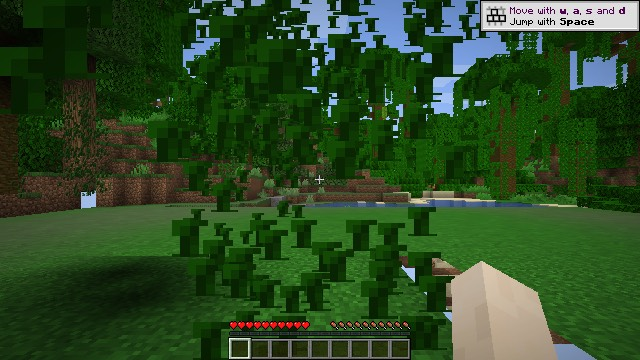
\includegraphics[width=0.48\linewidth]{frames/navigate_landmark-start.jpg}\hfill
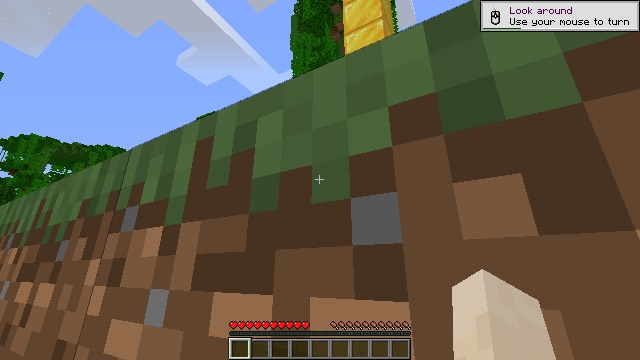
\includegraphics[width=0.48\linewidth]{frames/navigate_landmark-end.jpg}
\caption*{\textbf{navigate\_landmark} (navigation, fail (time)).
Goal: ``Walk to the gold pillar and stand next to it.'' Fable got within 3 blocks of the pillar (2.5 needed), sprinted past it, fell into a trench at the arena edge, and spent the rest of the time trying to dig out.}
\end{figure}

\begin{figure}[H]\centering
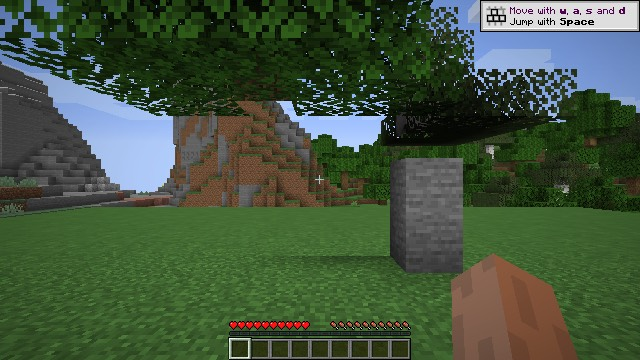
\includegraphics[width=0.48\linewidth]{frames/navigate_climb-start.jpg}\hfill
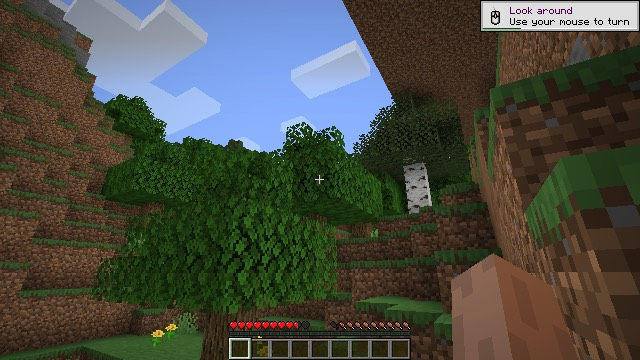
\includegraphics[width=0.48\linewidth]{frames/navigate_climb-end.jpg}
\caption*{\textbf{navigate\_climb} (navigation, fail (time)).
Goal: ``Climb the stone staircase in front of you and stand on top of the platform.'' Fable sprint-jumped toward the staircase, ended up inside tree leaves, then climbed a natural dirt hill instead and lost the staircase.}
\end{figure}

\begin{figure}[H]\centering
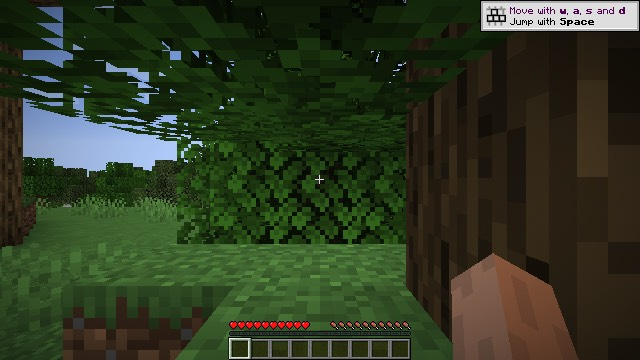
\includegraphics[width=0.48\linewidth]{frames/navigate_wall-start.jpg}\hfill
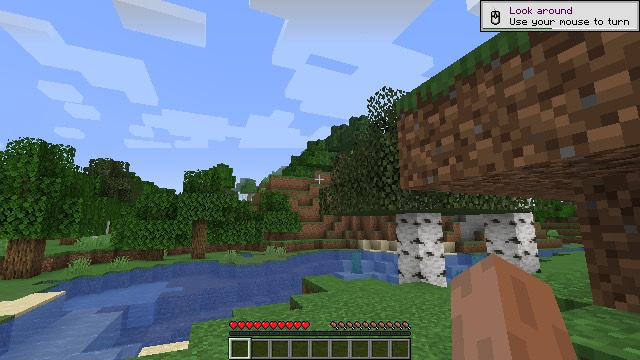
\includegraphics[width=0.48\linewidth]{frames/navigate_wall-end.jpg}
\caption*{\textbf{navigate\_wall} (navigation, fail (time)).
Goal: ``Get to the gold pillar behind the stone wall and stand next to it.'' Fable started around the edge of the wall, lost sight of it, and spent its last 15 decisions turning in place looking for it.}
\end{figure}

\begin{figure}[H]\centering
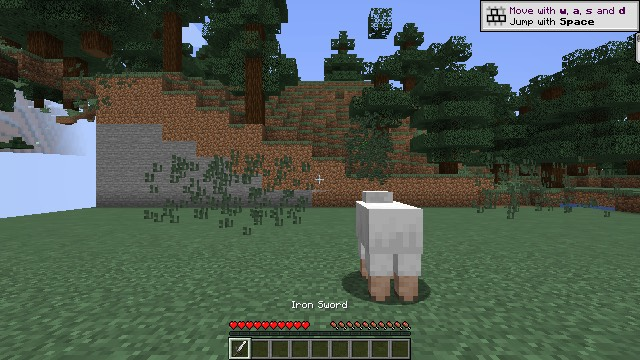
\includegraphics[width=0.48\linewidth]{frames/combat_sheep-start.jpg}\hfill
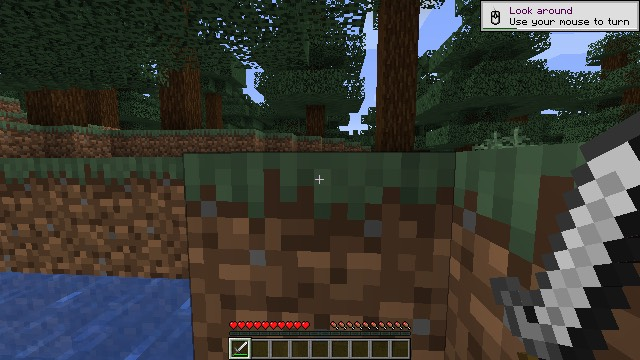
\includegraphics[width=0.48\linewidth]{frames/combat_sheep-end.jpg}
\caption*{\textbf{combat\_sheep} (combat, fail (time)).
Goal: ``Kill the sheep with your sword.'' Fable reached the sheep and swung 3 times, but the sheep left the screen (most likely fleeing after a hit) and Fable chased a far-off white shape until time ran out.}
\end{figure}

\begin{figure}[H]\centering
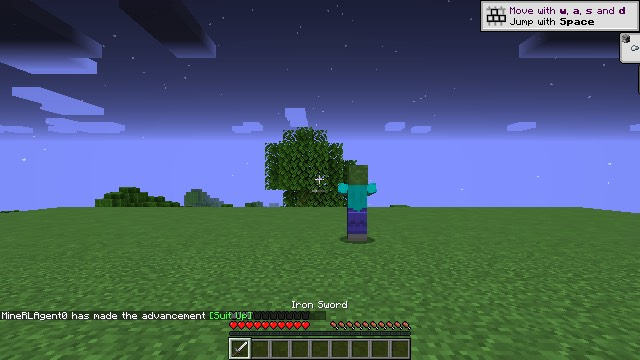
\includegraphics[width=0.48\linewidth]{frames/combat_zombie-start.jpg}\hfill
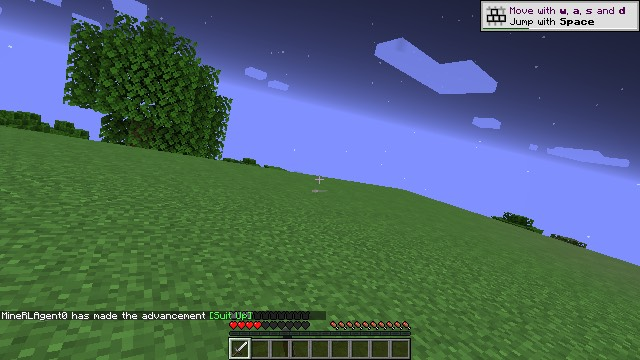
\includegraphics[width=0.48\linewidth]{frames/combat_zombie-end.jpg}
\caption*{\textbf{combat\_zombie} (combat, fail (died)).
Goal: ``Kill the zombie using your iron sword. Do not die.'' Fable traded hits with the zombie for 3 decisions and died after about 11 seconds, because the zombie kept hitting during each 3--4 s think.}
\end{figure}

\begin{figure}[H]\centering
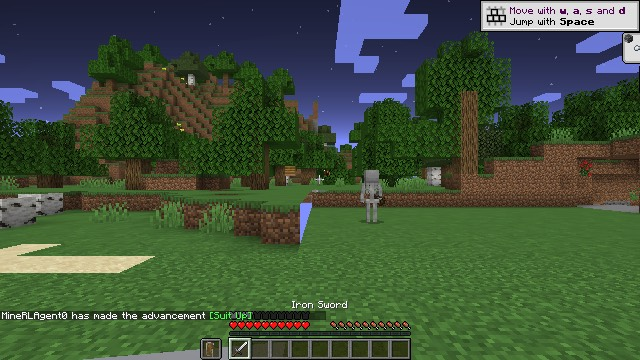
\includegraphics[width=0.48\linewidth]{frames/combat_skeleton-start.jpg}\hfill
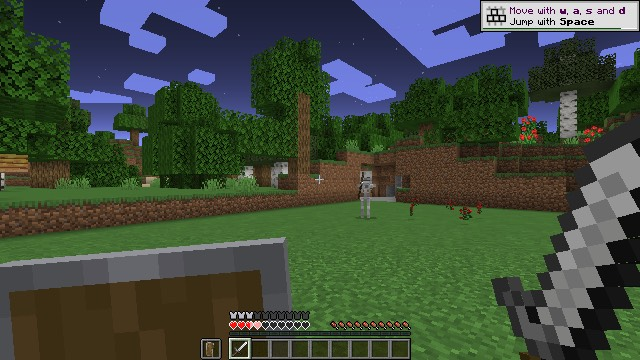
\includegraphics[width=0.48\linewidth]{frames/combat_skeleton-end.jpg}
\caption*{\textbf{combat\_skeleton} (combat, fail (died)).
Goal: ``Kill the skeleton. It shoots arrows. You have a sword, a shield, and armor.'' Fable chased the skeleton across a ledge while being shot and died before closing the distance.}
\end{figure}

\begin{figure}[H]\centering
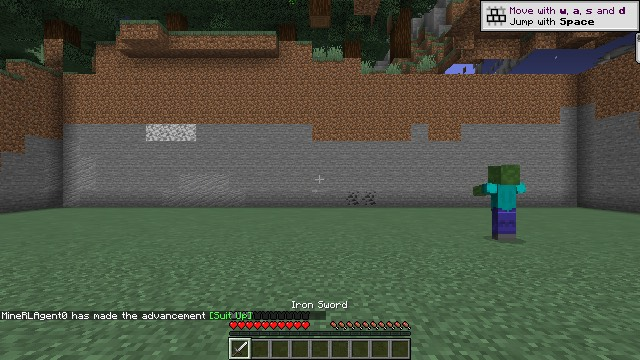
\includegraphics[width=0.48\linewidth]{frames/survive_one_zombie-start.jpg}\hfill
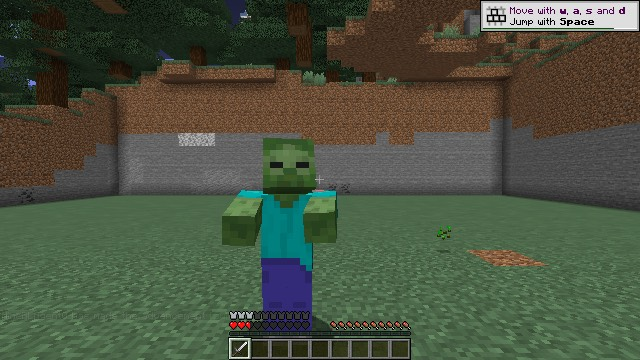
\includegraphics[width=0.48\linewidth]{frames/survive_one_zombie-end.jpg}
\caption*{\textbf{survive\_one\_zombie} (survival, fail (died)).
Goal: ``Stay alive for 30 seconds. A zombie is nearby. You have a sword and armor.'' Fable fought the zombie at close range while backing off, took hits faster than it could react, and died after 11 seconds.}
\end{figure}

\begin{figure}[H]\centering
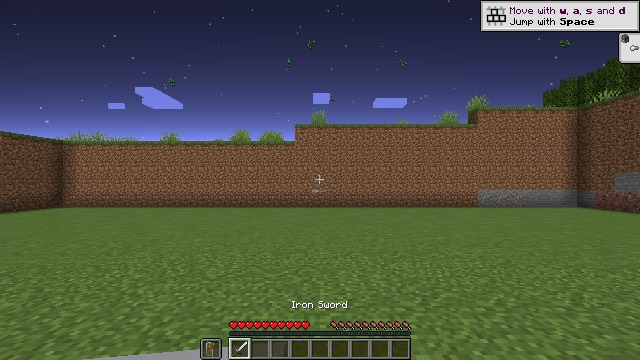
\includegraphics[width=0.48\linewidth]{frames/survive_mobs-start.jpg}\hfill
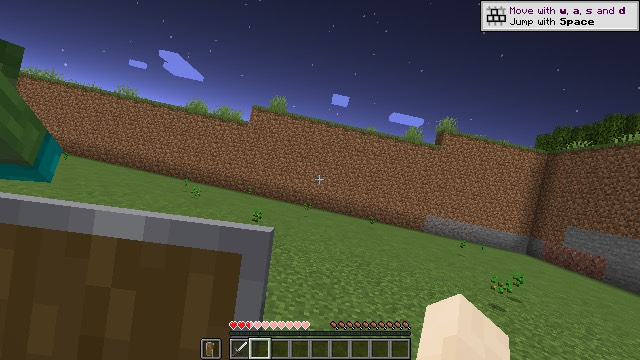
\includegraphics[width=0.48\linewidth]{frames/survive_mobs-end.jpg}
\caption*{\textbf{survive\_mobs} (survival, fail (died)).
Goal: ``Stay alive for 45 seconds. Zombies are coming. You have a sword and a shield.'' Fable scanned for the zombies, then fought them at close range once they arrived and died after 9 seconds.}
\end{figure}

\begin{figure}[H]\centering
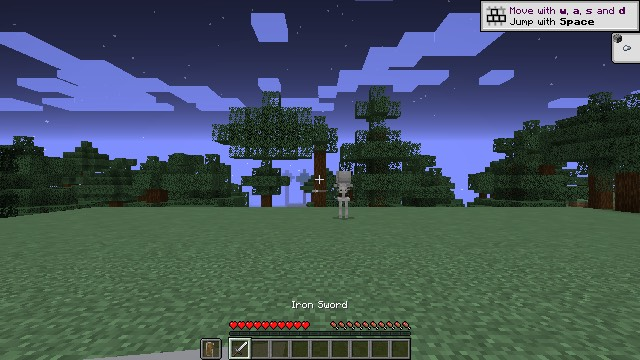
\includegraphics[width=0.48\linewidth]{frames/survive_skeletons-start.jpg}\hfill
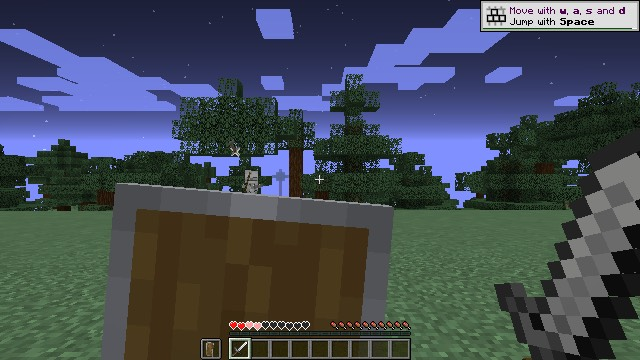
\includegraphics[width=0.48\linewidth]{frames/survive_skeletons-end.jpg}
\caption*{\textbf{survive\_skeletons} (survival, fail (died)).
Goal: ``Stay alive for 45 seconds. Two skeletons are shooting at you. You have a shield.'' Fable raised its shield toward one skeleton while the second skeleton kept shooting it from another side, and it died after 10 seconds.}
\end{figure}

\begin{figure}[H]\centering
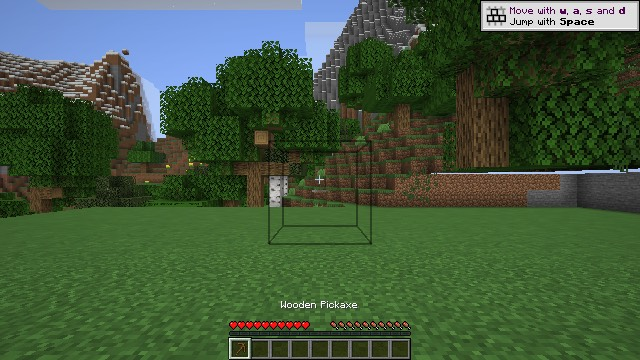
\includegraphics[width=0.48\linewidth]{frames/mine_stone-start.jpg}\hfill
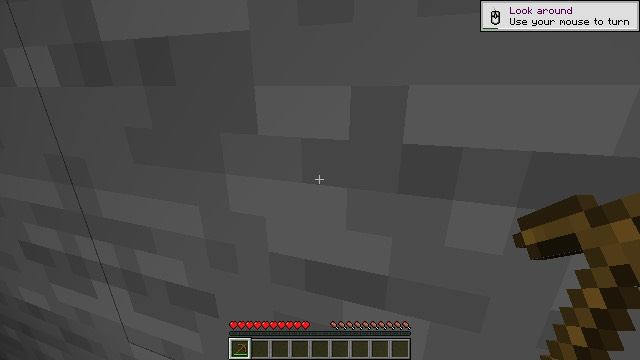
\includegraphics[width=0.48\linewidth]{frames/mine_stone-end.jpg}
\caption*{\textbf{mine\_stone} (manipulation, \textbf{pass}).
Goal: ``Mine 3 stone blocks with your pickaxe. The stone is in front of you.'' Passed: Fable walked to the stone, held attack on it, and mined 3 blocks.}
\end{figure}

\begin{figure}[H]\centering
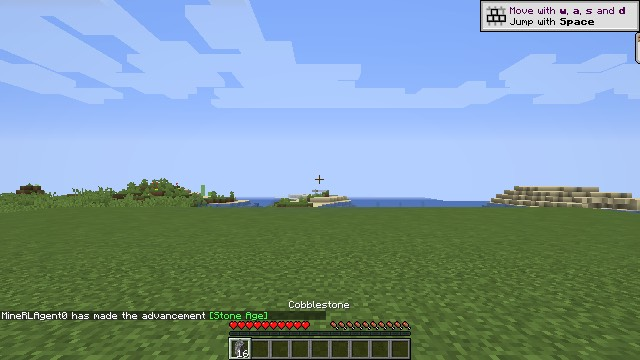
\includegraphics[width=0.48\linewidth]{frames/build_pillar-start.jpg}\hfill
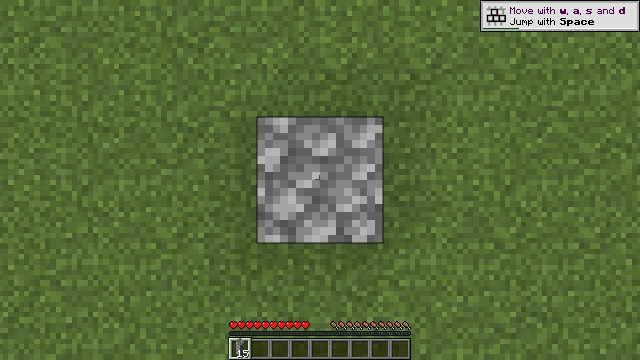
\includegraphics[width=0.48\linewidth]{frames/build_pillar-end.jpg}
\caption*{\textbf{build\_pillar} (manipulation, \textbf{pass}).
Goal: ``Build a pillar under yourself and stand at least 3 blocks above the ground. Place blocks while jumping.'' Passed: Fable looked straight down and jumped while placing cobblestone.}
\end{figure}

\begin{figure}[H]\centering
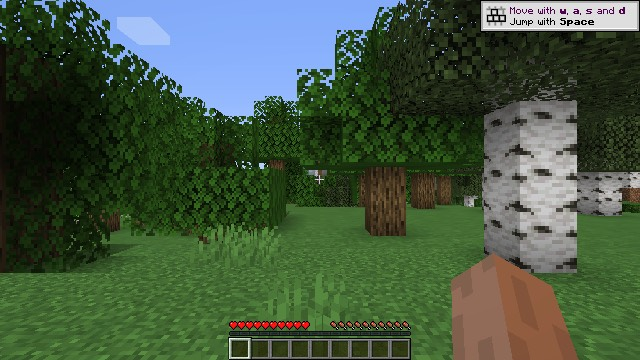
\includegraphics[width=0.48\linewidth]{frames/explore_behind-start.jpg}\hfill
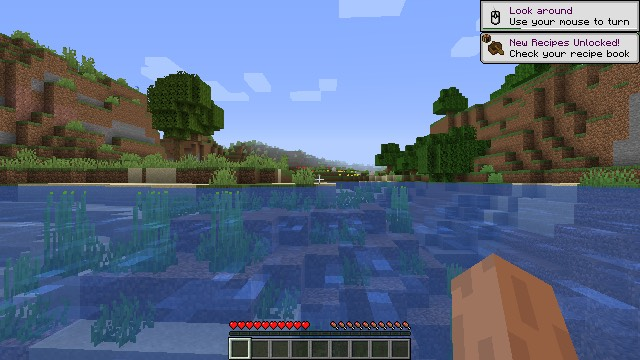
\includegraphics[width=0.48\linewidth]{frames/explore_behind-end.jpg}
\caption*{\textbf{explore\_behind} (exploration, fail (time)).
Goal: ``Find the diamond block pillar somewhere around you and stand next to it.'' Fable never saw the diamond pillar, headed for something it thought it saw on the horizon, and ended up swimming across a lake.}
\end{figure}

\begin{figure}[H]\centering
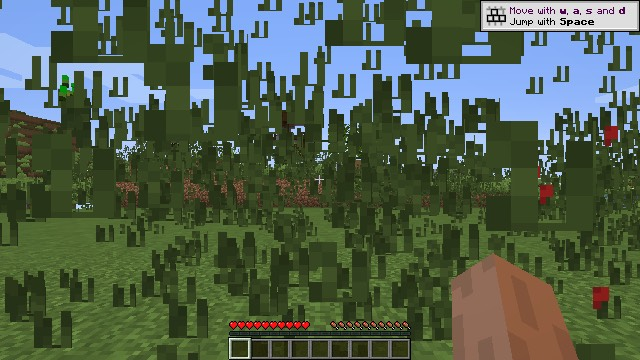
\includegraphics[width=0.48\linewidth]{frames/explore_visit_two-start.jpg}\hfill
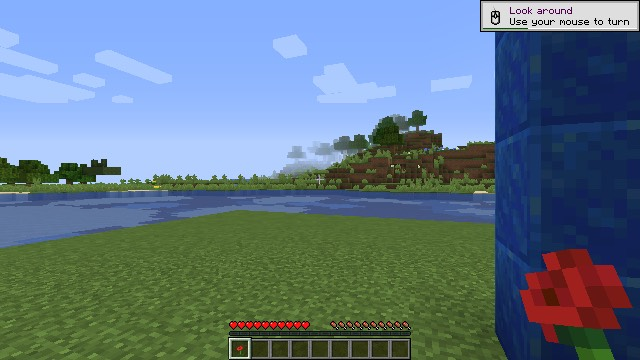
\includegraphics[width=0.48\linewidth]{frames/explore_visit_two-end.jpg}
\caption*{\textbf{explore\_visit\_two} (exploration, \textbf{pass}).
Goal: ``There is a gold pillar and a lapis pillar somewhere around you. Visit both. Order does not matter.'' Passed: Fable found the gold pillar first, scanned until it saw the lapis pillar, and walked to it.}
\end{figure}

\begin{figure}[H]\centering
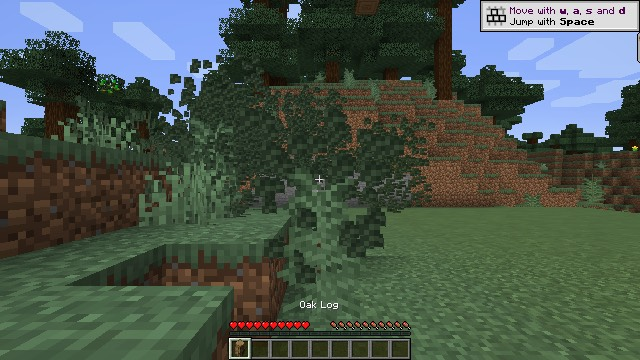
\includegraphics[width=0.48\linewidth]{frames/craft_planks-start.jpg}\hfill
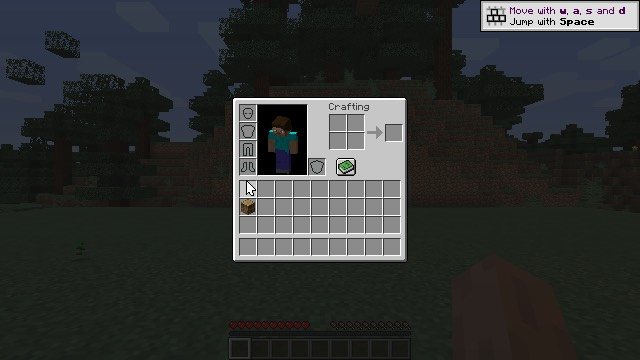
\includegraphics[width=0.48\linewidth]{frames/craft_planks-end.jpg}
\caption*{\textbf{craft\_planks} (planning, fail (time)).
Goal: ``Turn the log in your inventory into wooden planks. Open your inventory with the inventory key.'' Fable opened the inventory but could not land the mouse cursor on the log, missing it on every try.}
\end{figure}

\begin{figure}[H]\centering
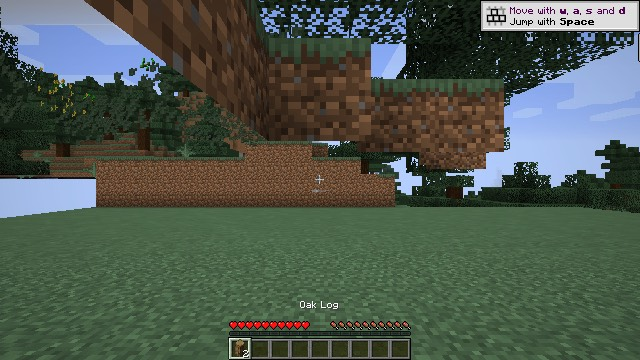
\includegraphics[width=0.48\linewidth]{frames/craft_table-start.jpg}\hfill
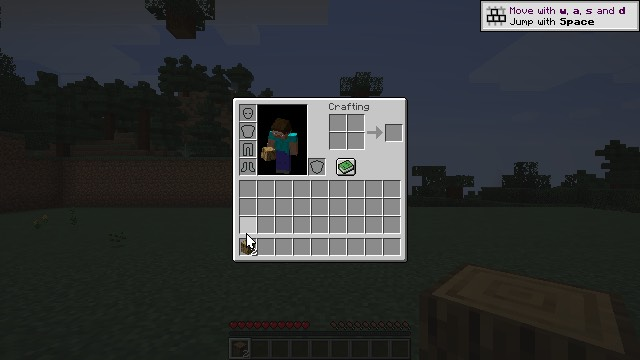
\includegraphics[width=0.48\linewidth]{frames/craft_table-end.jpg}
\caption*{\textbf{craft\_table} (planning, fail (time)).
Goal: ``Craft a crafting table using the logs in your inventory. Open your inventory with the inventory key.'' Fable could not land the mouse cursor on the logs, the same problem as craft\_planks.}
\end{figure}

\begin{figure}[H]\centering
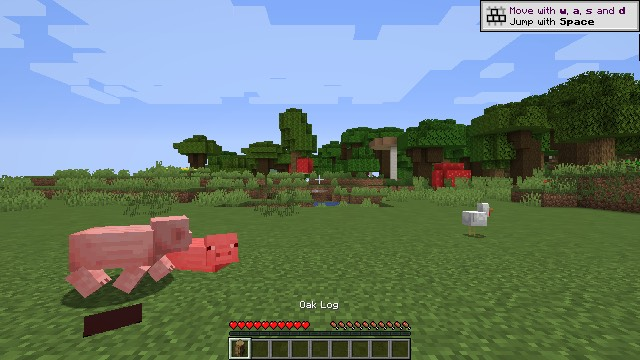
\includegraphics[width=0.48\linewidth]{frames/craft_sticks-start.jpg}\hfill
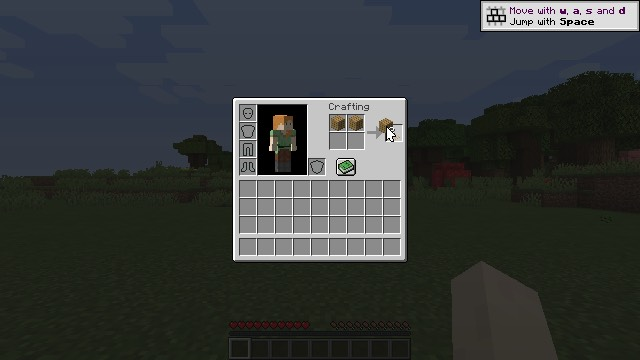
\includegraphics[width=0.48\linewidth]{frames/craft_sticks-end.jpg}
\caption*{\textbf{craft\_sticks} (planning, fail (time)).
Goal: ``Craft at least 4 sticks starting from the log in your inventory. Open your inventory with the inventory key.'' Fable turned the log into planks but ran out of time while arranging planks in the crafting grid.}
\end{figure}

\begin{figure}[H]\centering
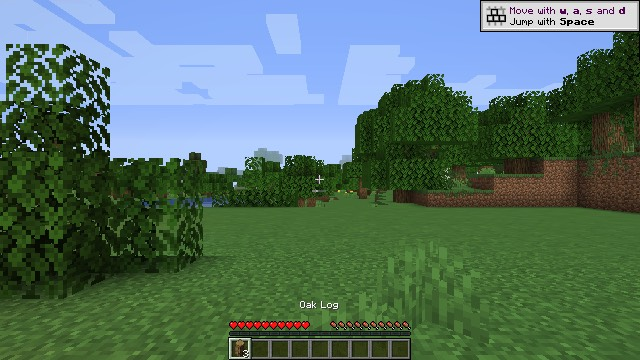
\includegraphics[width=0.48\linewidth]{frames/craft_pickaxe-start.jpg}\hfill
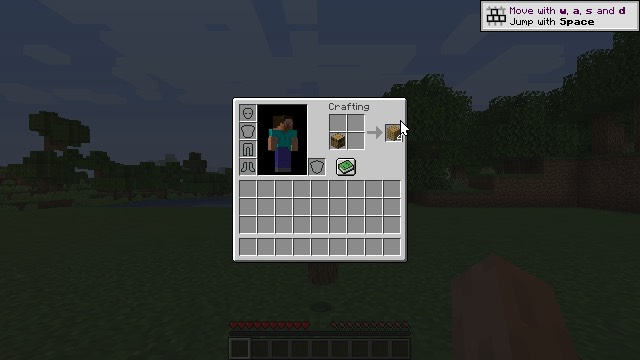
\includegraphics[width=0.48\linewidth]{frames/craft_pickaxe-end.jpg}
\caption*{\textbf{craft\_pickaxe} (planning, fail (time)).
Goal: ``Craft a wooden pickaxe. You start with logs. You will need a crafting table.'' Fable spent all 150 seconds moving logs and planks around the inventory and never got past making planks.}
\end{figure}

\begin{figure}[H]\centering
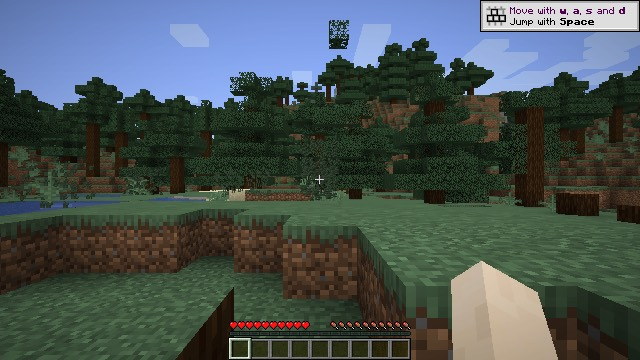
\includegraphics[width=0.48\linewidth]{frames/adapt_target_moves-start.jpg}\hfill
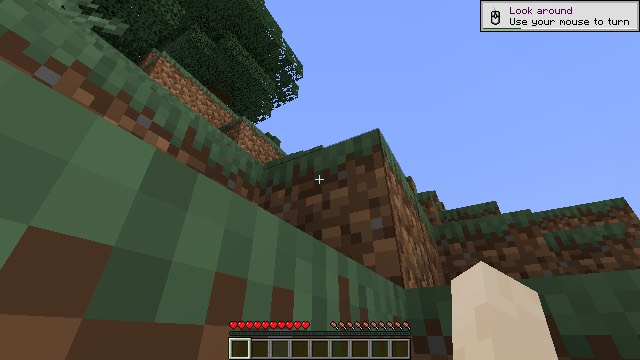
\includegraphics[width=0.48\linewidth]{frames/adapt_target_moves-end.jpg}
\caption*{\textbf{adapt\_target\_moves} (adaptation, fail (time)).
Goal: ``Walk to the gold pillar and stand next to it. The pillar may move.'' Fable lost sight of the pillar behind trees and spent its last decisions trying to climb a dirt cliff toward where it guessed the pillar was.}
\end{figure}

\begin{figure}[H]\centering
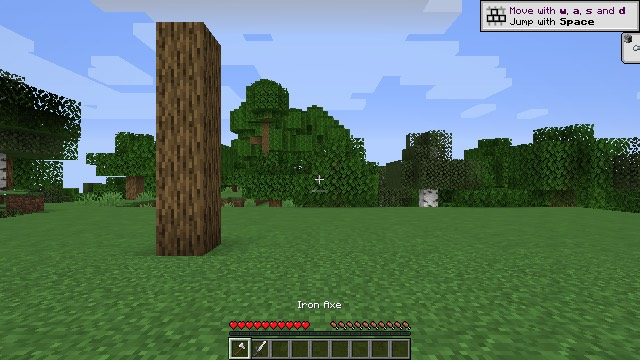
\includegraphics[width=0.48\linewidth]{frames/adapt_night_falls-start.jpg}\hfill
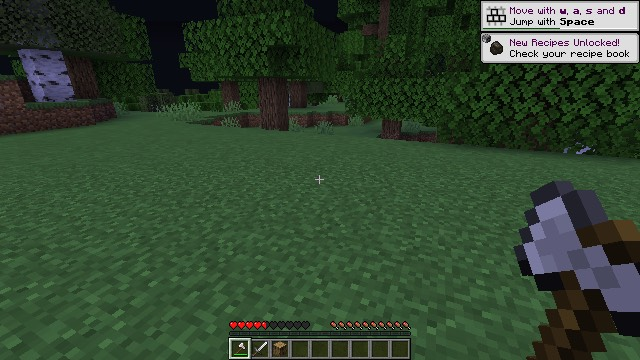
\includegraphics[width=0.48\linewidth]{frames/adapt_night_falls-end.jpg}
\caption*{\textbf{adapt\_night\_falls} (adaptation, fail (died)).
Goal: ``Collect 3 wood logs from the log pillar and pick them up. Watch out, things may change.'' Fable chopped 2 logs, lost the pillar when night fell, and was killed by mobs before finding it again.}
\end{figure}
\end{document}
